\documentclass{article}
\usepackage[utf8]{inputenc}
\usepackage{amsmath}
\usepackage{listings}
\usepackage{color}
\usepackage{float}
\usepackage{hyperref}
\usepackage{graphicx}
\usepackage{caption}
\usepackage{subcaption}
\usepackage{adjustbox}
\pagestyle{empty}
\usepackage{listings}
\usepackage[a4paper, total={7in, 9in}]{geometry}

\graphicspath{{/Users/ritz/Necessity/MSU/Courses/1st Year/Spring 2021/CSE 848 Evolutionary Computation/Assignments/HA4/Codes/}}

\definecolor{codebg}{gray}{0.95}

\lstset{ 
	language=Matlab,                		% choose the language of the code
	%	basicstyle=10pt,       				% the size of the fonts that are used for the code
	numbers=left,                  			% where to put the line-numbers
	numberstyle=\footnotesize,      		% the size of the fonts that are used for the line-numbers
	stepnumber=1,                   			% the step between two line-numbers. If it's 1 each line will be numbered
	numbersep=5pt,                  		% how far the line-numbers are from the code
	backgroundcolor=\color{codebg},  	% choose the background color. You must add \usepackage{color}
	showspaces=false,               		% show spaces adding particular underscores
	showstringspaces=false,         		% underline spaces within strings
	showtabs=false,                 			% show tabs within strings adding particular underscores
	%	frame=single,	                			% adds a frame around the code
	%	tabsize=2,                				% sets default tabsize to 2 spaces
	%	captionpos=b,                   			% sets the caption-position to bottom
	breaklines=true,                			% sets automatic line breaking
	breakatwhitespace=false,        		% sets if automatic breaks should only happen at whitespace
	escapeinside={\%*}{*)}          		% if you want to add a comment within your code
}

\title{\textbf{CSE 848 Home Assignment 4}}
\author{\textbf{\textit{Submitted by:}} Ritam Guha (MSU ID: guharita)}
\date{\textbf{\textit{Date:}} March 15, 2021}

\begin{document}
	
	\maketitle
	
	\section{Question}
	Write a binary-coded genetic algorithm (BGA) with binary tournament selection operator, one-point crossover operator and bit-wise mutation operators. No elite preservation is to be used. Apply the BGA code to solve two, 30-variable maximization problems constructed from 10, three-bit substrings ($s_i, i = 1, 2, . . . , 10$). The structure of the overall function is given below:
	\begin{equation}
		\displaystyle F(s) = 10 \sum_{i=1}^1 f(s_i)
	\end{equation}

	where 30-bit string s is constructed from 10, three-bit substrings as $s = (s_1 \cup s_2 \cup · · · \cup s_10$). Two subfunctions as a function of three bits are defined below:\\
	
	
	\textbf{Problem 1:} The subfunction f is a function of unitation u, defined as the number of $1$s in the three-bit substring: $f(u) = u/3$. For example, $f(011) = f(101) = f(110) = 2/3 = 0.67$, as for these three substrings $u = 2$.\\
	
	\textbf{Problem2:} $f(u)=0.9-u/3$ for $u<3$, and $f(3)=1$.\\
	
	Notice that for both problems, the optimal string is the all-1 string $s\text{*} =(111 . . . 1)$ having $F (s\text{*} )=100$.\\
	
	Two construction procedures are used:\\
	
	\textbf{Construction 1:} The first three bits of $s$ are used to construct the first subproblem, the next three bits of $s$ are used to construct the second subproblem, and so on. Thus, the final three bits ($28^{th}$, $29^{th}$ and $30^{th}$ bits) are used to construct $10^{th}$ subfunction.\\
	
	\textbf{Construction2:} $1^{st}$,$11^{th}$ and $21^{st}$ bits of $s$ are used to construct the first subproblem,then $2^{nd}$, $12^{th}$ and $22^{nd}$ bits of $s$ are used to construct the second subproblem, and so on. The $10^{th}$ subfunction uses $10^{th}$, $20^{th}$ and $30^{th}$ bits of $s$.\\
	
	\hrule  
	\vspace{2mm}
		
	\textbf{Response:}\\
	
	The given problem can be treated as an engineering function optimization problem where the function is given by $F(s)$. It is a maximization problem where the goal is to maximize the given function.\\
	
	\subsection{Solution Formulation}
	A Binary Genetic Algorithm (BGA) is used to solve this engineering function optimization problem. The fitness function for the BGA is the engineering function mentioned as $F(s)$. For 2 constructions and 2 problems, we have $(2 \times 2) = 4$ different objective function formulations.\\
	
	The BGA consists of evolutionary operators like mutation, crossover and binary tournament selection. No elitist preservation strategy is to be used for solving these problems.\\
	
	The hyperparameter combination used for constructing the BGA is provided in the following Table:\\
	
	\begin{table}[H]
		\centering
		\begin{tabular}{|c|c|}
			\hline
			\textbf{Hyper-parameter} & \textbf{Value} \\ \hline
			Number of Chromosomes & 60 \\ 
			Number of Generations & 200 \\
			Mutation Rate & $\displaystyle \frac{1}{30}$ \\ 
			Crossover Rate & 0.9 \\ 
			Number of Runs & 30 \\ \hline
		\end{tabular}
	\caption{Hyperparameter combination used for the BGA}
	\end{table}
	
	\subsection{Code}
	 The BGA code used for this procedure is shown below:
	 \lstinputlisting[language=Python]{Codes/BGA.py}
	 
	 \vspace{5mm}
	 
	The main function running the BGA code is presented below:
	\lstinputlisting[language=Python]{Codes/main.py}
	
	\vspace{2mm}
	By running the code over 4 combinations of (problem, construction), I obtained the following results:\\
	
	\begin{table}[H]
		\centering
		\caption{Best, Median, Mean and Worst objective value obtained for 30 runs of BGA over different problem-construction settings.}
		\begin{tabular}{|c|c|c|c|c|}
			\hline
			\textbf{Problem Statement} & \textbf{Best}  & \textbf{Median} & \textbf{Mean} & \textbf{Worst} \\ \hline
			Problem-1 Construction-1 & 100 & 93.33 & 94.67 & 90 \\ \hline
			Problem-1 Construction-2 & 100 & 93.33 & 94.44 & 90 \\ \hline
			Problem-2 Construction-1 & 97 & 91.67 & 91.7 & 88.33 \\ \hline
			Problem-2 Construction-2 & 96 & 90 & 90.01 & 84.33 \\ \hline
		\end{tabular}
	\end{table}
	
	From the results, it is clear than Problem-1 is relatively easier to solve, while Problem-2 is harder. The code could not get to the global optimum solution for problem 2. Construction-wise, the result shows that construction 1 is easier to follow than construction 2.\\
	
	Now let us discuss the problem-construction setting-wise discussion of BGA.\\
	
	\subsection{Problem-1}
	Problem 1 is easier to solve. This is because problem 1 only focuses on increasing the number of 1's in the candidate solutions and the global maximum is present at the position where all the variables are 1s. So, here, we can use some guidance from the better solutions (Here better solutions are the ones having more number of 1s) in forms of recombination or selection to move towards the global maximum solution. This problem is excellent for checking the exploitation capabilities of the algorithm.
	
	\subsubsection{Construction-1}
	The goal of the 1st construction is to correlate variables which are placed closer to each other in the candidate solutions (testing the \textit{linkage} property). For Problem-1, Construction-1, the BGA I formulated worked really well and was able to achieve good performace in terms of the objective function. For the median run, out of all the 30 runs, the plot of the objective scores against the generations is presented below:
	
	\begin{figure}[H]
		\centering
		\includegraphics[scale=0.8]{Problem_1 Construction_1/Plot.jpg}
		\caption{The best and average objective scores for the generations of the median run of BGA}
		\label{Prob_1_Const_1_Plot}
	\end{figure}    
	
	From the plot, it is clear that, the algorithm always prefers better solutions over the course of generations. The best solution is always as good as the solution of the previous generation and sometimes better than that. Although the average objective score is fluctuating, in the long run, it is moving towards better objective scores.\\
	
	Another interesting thing to see over here is the count of different competiting schemas present in the population across all the generations. For this reason I have plotted the fraction of competiting schemas for every generation in the next Figure. In \autoref{Prob_1_Const_1_Comp_Plot}, 0(x) represents all 0s for subproblem x and 1(x) represents all 1s for subproblem x. So, these two are competiting schemas for subproblem x. As there are 10 subproblems in the given problem, we have 10 plots for competitors in the Figure. From the Figure, it is clear that the algorithm is prefering increasing number of 1s in the solutions over the 0s across different generations.\\
	
	\begin{figure}[H]
		\centering
		\begin{adjustbox}{width=0.6\paperwidth}
			\begin{tabular}{c c}
				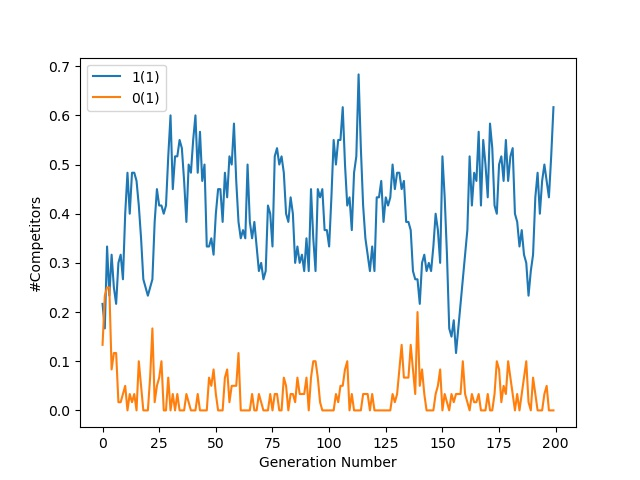
\includegraphics{Codes/Problem_1 Construction_1/Comp_1.jpg} & 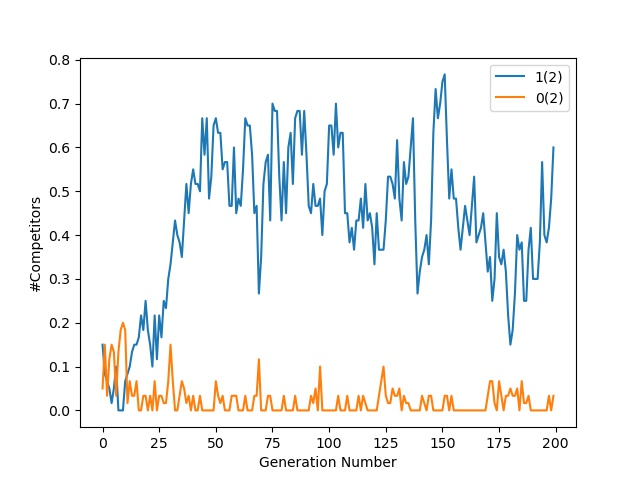
\includegraphics{Codes/Problem_1 Construction_1/Comp_2.jpg} \\
				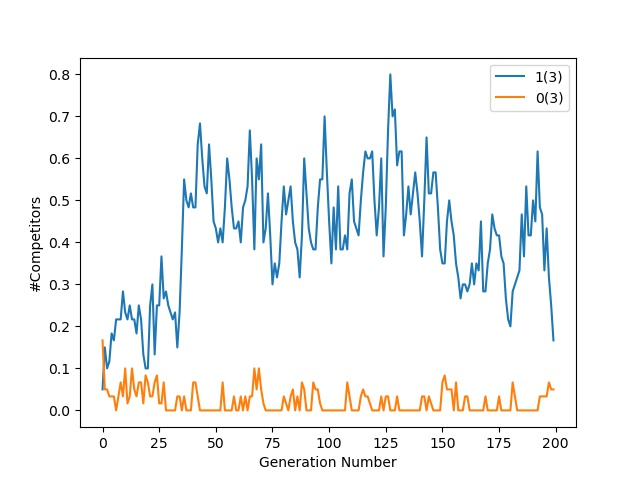
\includegraphics{Codes/Problem_1 Construction_1/Comp_3.jpg}&
				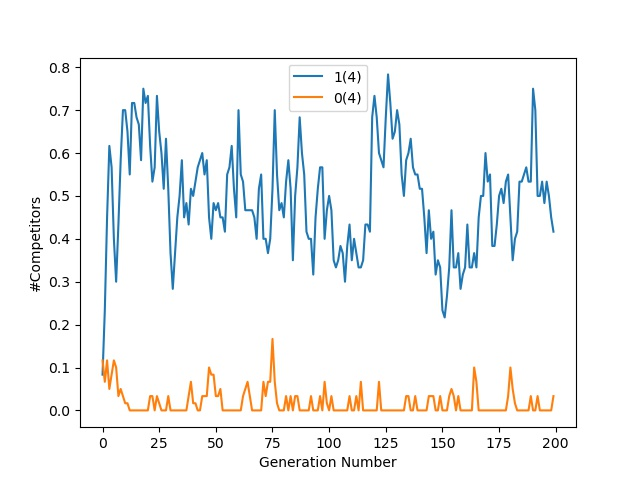
\includegraphics{Codes/Problem_1 Construction_1/Comp_4.jpg} \\ 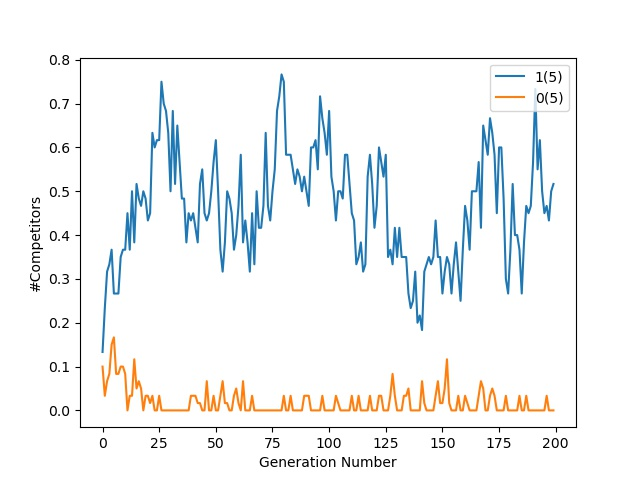
\includegraphics{Codes/Problem_1 Construction_1/Comp_5.jpg} &
				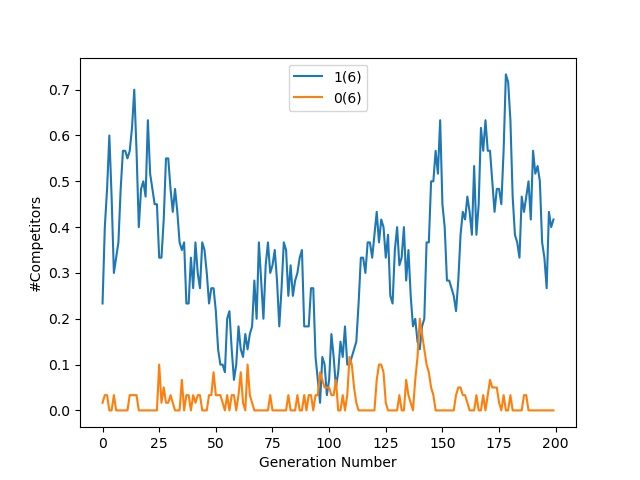
\includegraphics{Codes/Problem_1 Construction_1/Comp_6.jpg}\\
				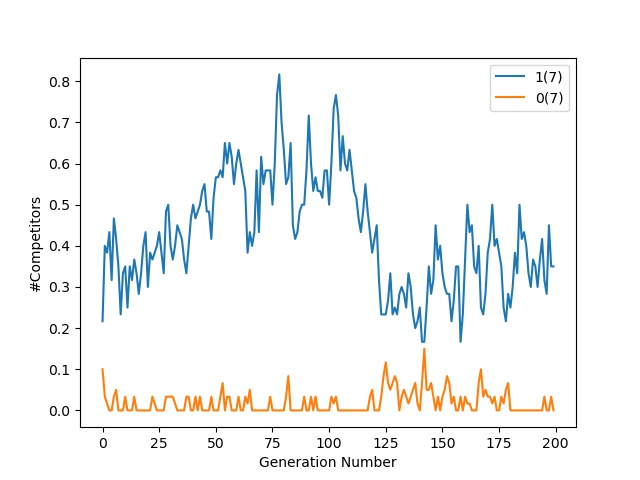
\includegraphics{Codes/Problem_1 Construction_1/Comp_7.jpg} & 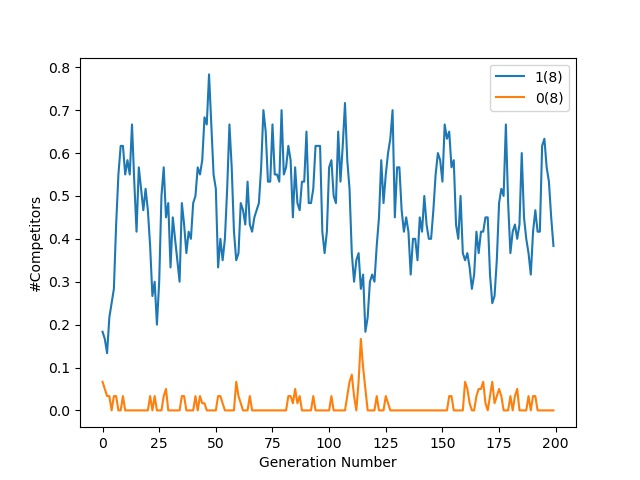
\includegraphics{Codes/Problem_1 Construction_1/Comp_8.jpg} \\
				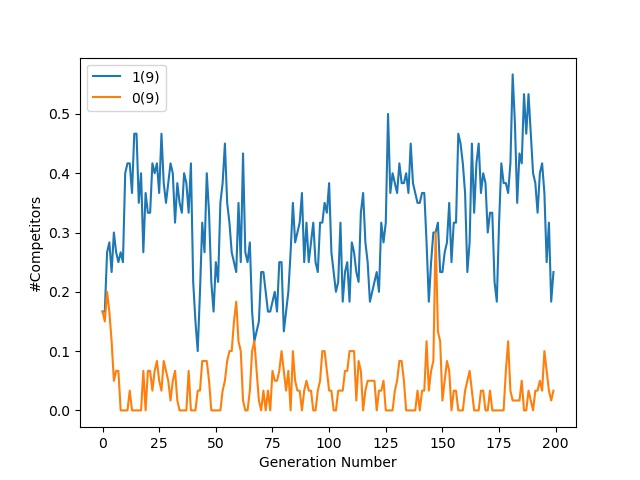
\includegraphics{Codes/Problem_1 Construction_1/Comp_9.jpg}&
				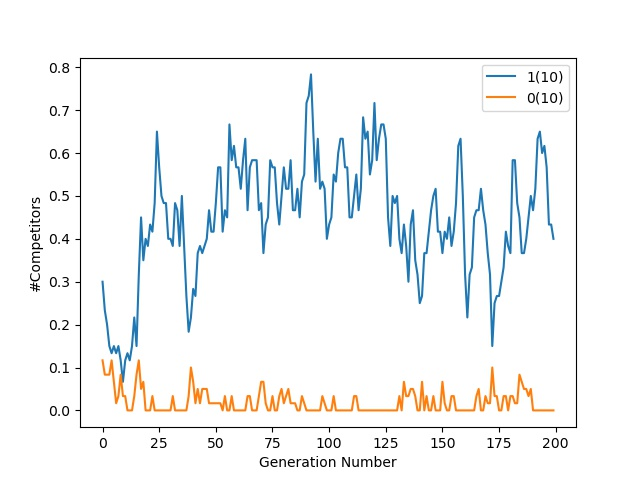
\includegraphics{Codes/Problem_1 Construction_1/Comp_10.jpg}\\
			\end{tabular}
		\end{adjustbox}
		\caption{Plot of fraction of competiting schemas across the generations of the median run. In the legend, 1(x) and 0(x) mean\ all 1s and all 0s for subproblem x respectively.}
		\label{Prob_1_Const_1_Comp_Plot}
	\end{figure}

	\subsubsection{Construction-2}
	
	Construction 2 tries to find distant relationships among variables. It takes variables at a distance of 10 from each other and combines them to provide the objective score. The goal of the construction is to model the concept of \textit{epistasis} through the algorithm.
	Construction 2 for Problem 1 provides similar results as Construction 1. The objective scores over the generations for this setting is presented in \autoref{Prob_1_Const_2_Plot}. The same trend of increasing objective score is observed in this plot too.
	
	\begin{figure}[H]
		\centering
		\includegraphics[scale=0.8]{Problem_1 Construction_2/Plot.jpg}
		\caption{The best and average objective scores for the generations of the median run of BGA}
		\label{Prob_1_Const_2_Plot}
	\end{figure}    
	
	The same trend is also continued in the schema competitors' plot which is shown in \autoref{Prob_1_Const_2_Comp_Plot}. 1s are getting same kind of importance over 0s in the candidate solutions over the course of iterations.
	\begin{figure}[H]
		\centering
		\begin{adjustbox}{width=0.6\paperwidth}
			\begin{tabular}{c c}
				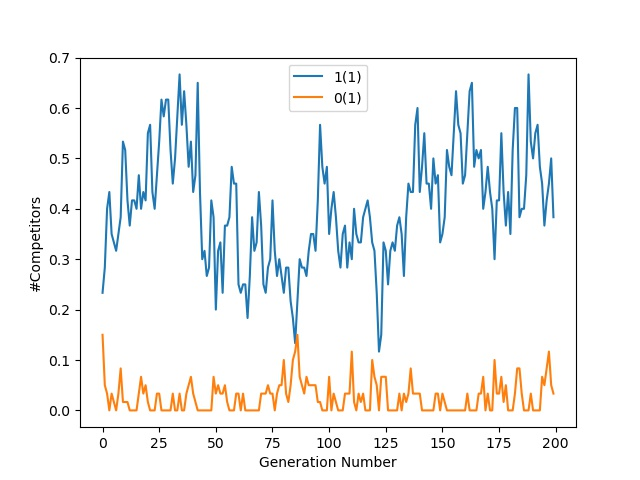
\includegraphics{Codes/Problem_1 Construction_2/Comp_1.jpg} & 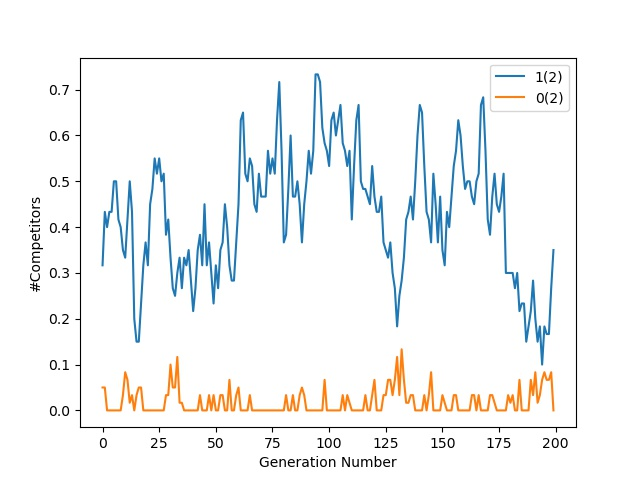
\includegraphics{Codes/Problem_1 Construction_2/Comp_2.jpg} \\
				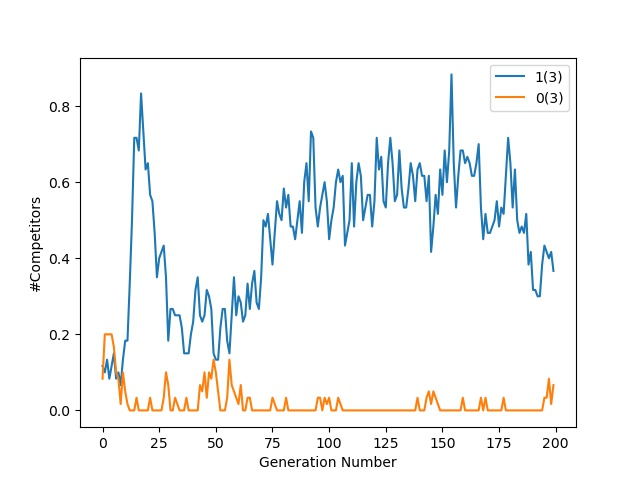
\includegraphics{Codes/Problem_1 Construction_2/Comp_3.jpg}&
				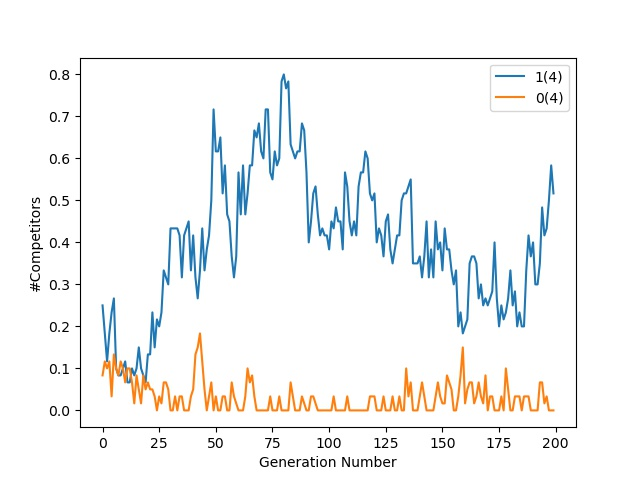
\includegraphics{Codes/Problem_1 Construction_2/Comp_4.jpg} \\ 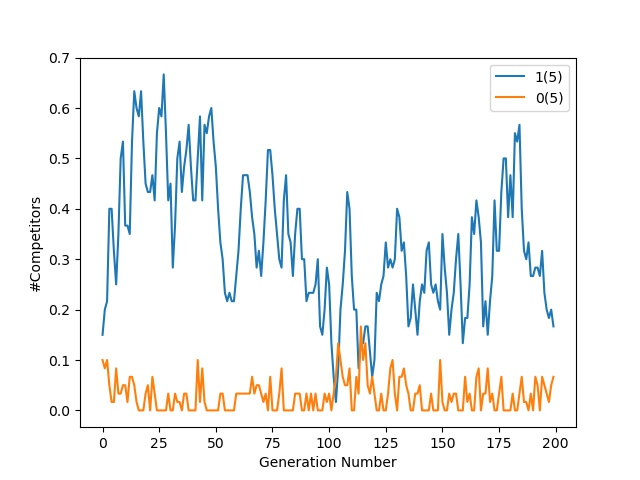
\includegraphics{Codes/Problem_1 Construction_2/Comp_5.jpg} &
				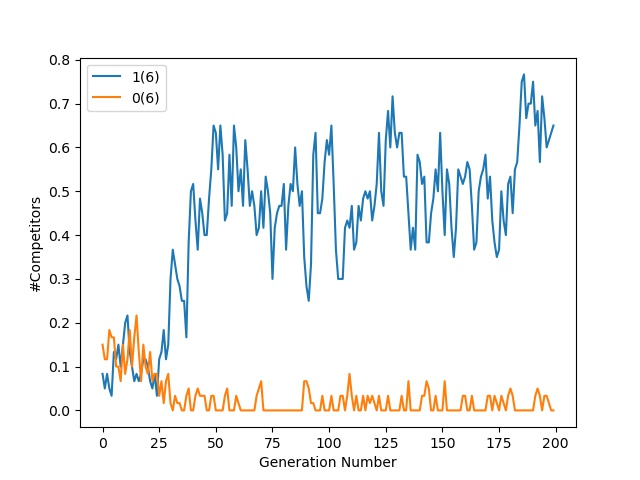
\includegraphics{Codes/Problem_1 Construction_2/Comp_6.jpg}\\
				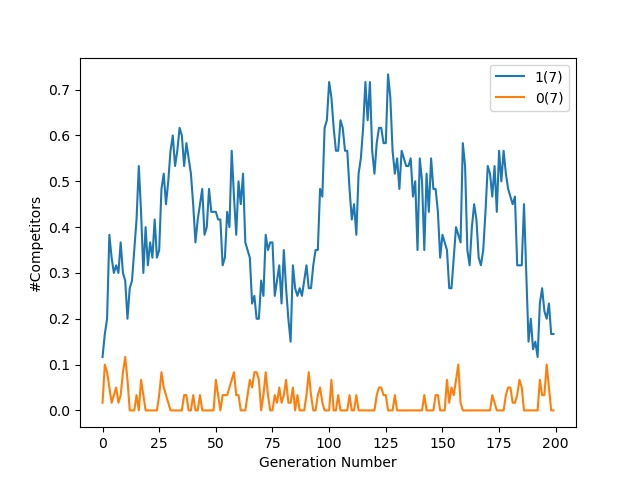
\includegraphics{Codes/Problem_1 Construction_2/Comp_7.jpg} & 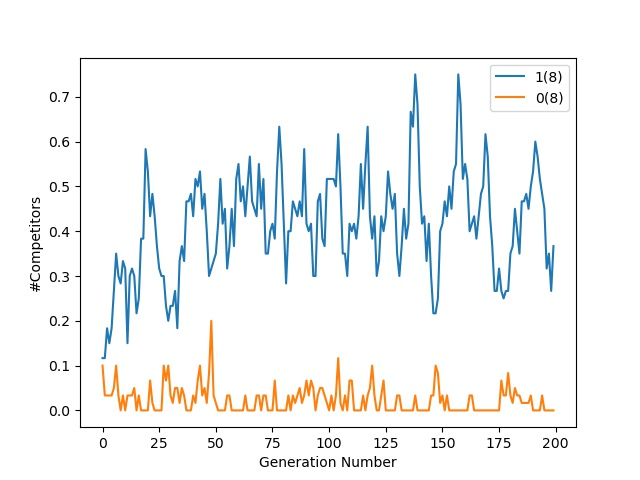
\includegraphics{Codes/Problem_1 Construction_2/Comp_8.jpg} \\
				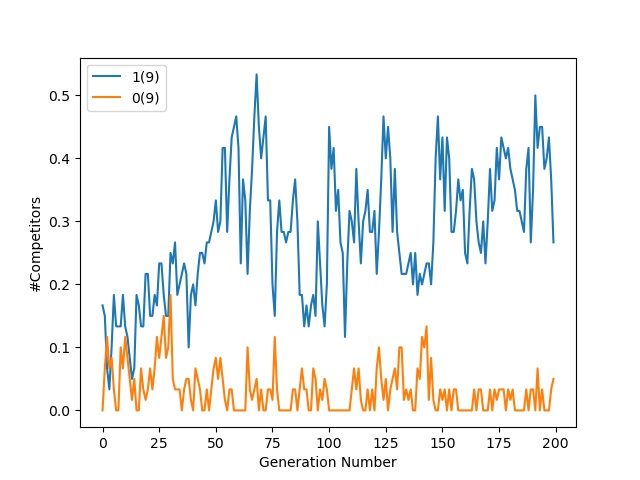
\includegraphics{Codes/Problem_1 Construction_2/Comp_9.jpg}&
				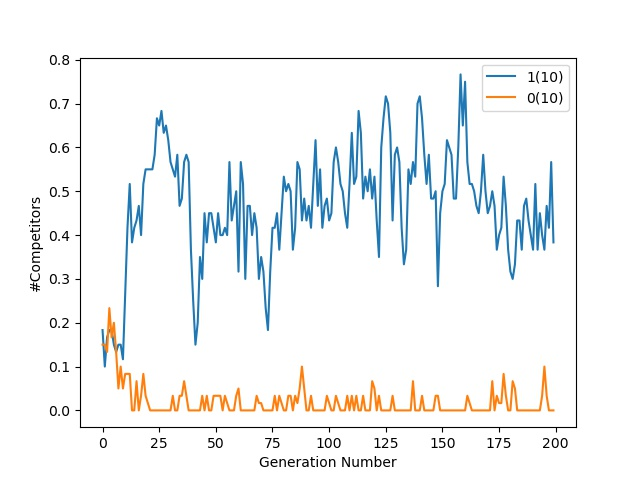
\includegraphics{Codes/Problem_1 Construction_2/Comp_10.jpg}\\
			\end{tabular}
		\end{adjustbox}

		\caption{Plot of fraction of competiting schemas across the generations of the median run. In the legend, 1(x) and 0(x) mean\ all 1s and all 0s for subproblem x respectively.}
		\label{Prob_1_Const_2_Comp_Plot}
	\end{figure}

\subsection{Problem-2}
Problem 2 is more complicated than Problem 1. In problem 2, 0s are preferred over 1s unless a subproblem has all 1s in its variables. This makes the situation worse because the problem formulation guides solution towards the direction opposite to the direction of the global maximum unless a solution is able to randomly find the global maximum. This problem focuses more on the explorational capabilities of the algorithm under consideration.

\subsubsection{Construction-1}
In \autoref{Prob_2_Const_1_Plot}, we can see that the algorithm is still able to find decent solutions over the course of generations. But it was not able to achieve the best objective score. So, it could not get to the global maximum solution. This shows the deceptive nature of the problem 2.
\begin{figure}[H]
	\centering
	\includegraphics[scale=0.8]{Problem_2 Construction_1/Plot.jpg}
	\caption{The best and average objective scores for the generations of the median run of BGA}
	\label{Prob_2_Const_1_Plot}
\end{figure}    

The interesting thing about problem 2 starts getting noticed when we move our discussion to the fraction of schemas getting preferred over the generations. From \autoref{Prob_2_Const_1_Comp_Plot}, it is visible how the algorithm got confused between selecting 1s and selecting 0s. Sometimes 0s got ahead of the 1s and sometimes it went the other way round for different subproblems. This trend is completely differnt from problem 1 which always favoured 1s over 0s. 

\begin{figure}[H]
	\centering
	\begin{adjustbox}{width=0.6\paperwidth}
		\begin{tabular}{c c}
			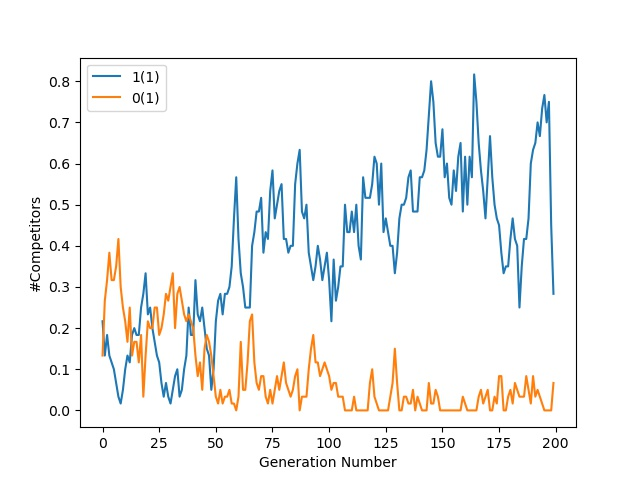
\includegraphics{Codes/Problem_2 Construction_1/Comp_1.jpg} & 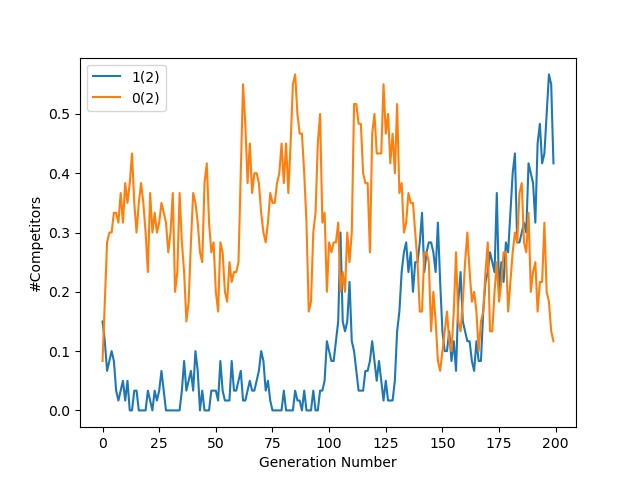
\includegraphics{Codes/Problem_2 Construction_1/Comp_2.jpg} \\
			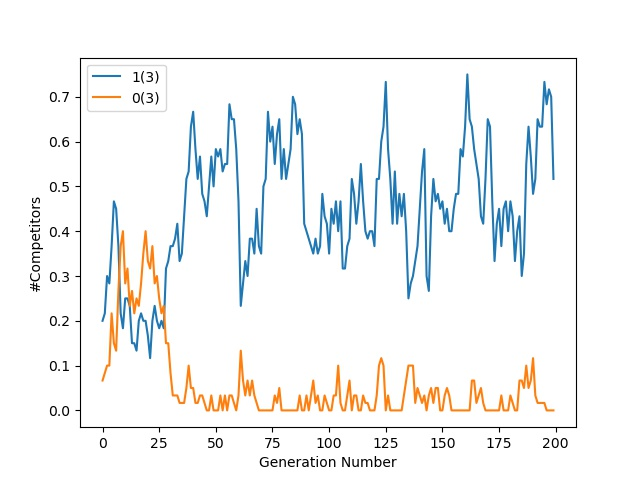
\includegraphics{Codes/Problem_2 Construction_1/Comp_3.jpg}&
			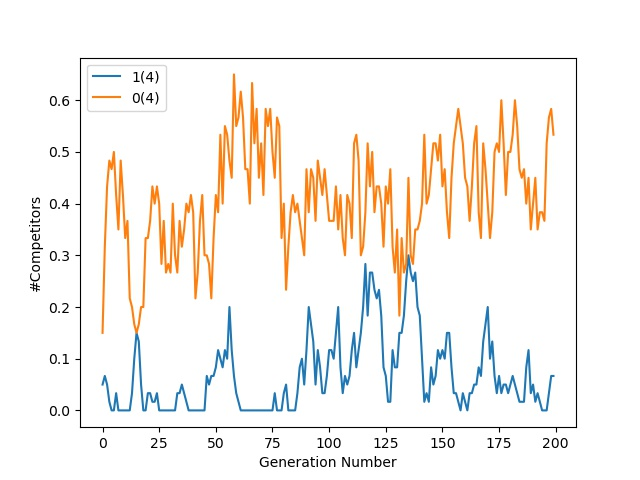
\includegraphics{Codes/Problem_2 Construction_1/Comp_4.jpg} \\ 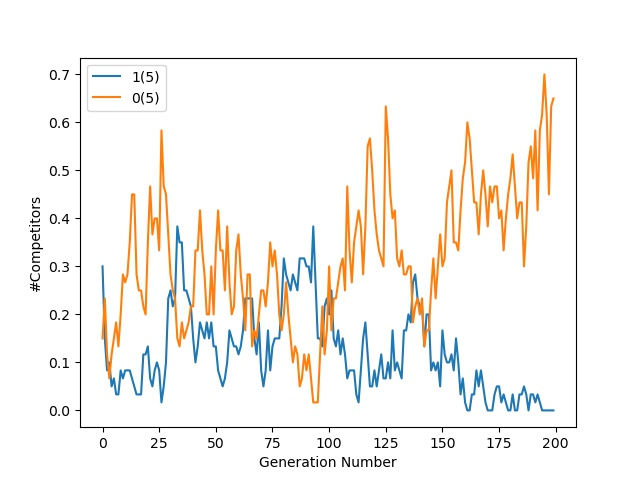
\includegraphics{Codes/Problem_2 Construction_1/Comp_5.jpg} &
			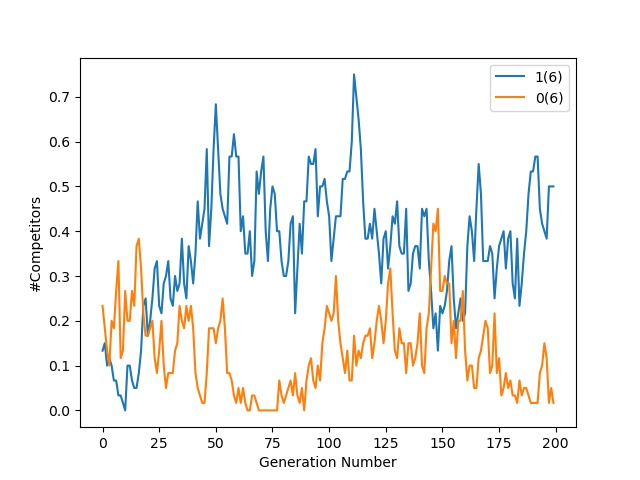
\includegraphics{Codes/Problem_2 Construction_1/Comp_6.jpg}\\
			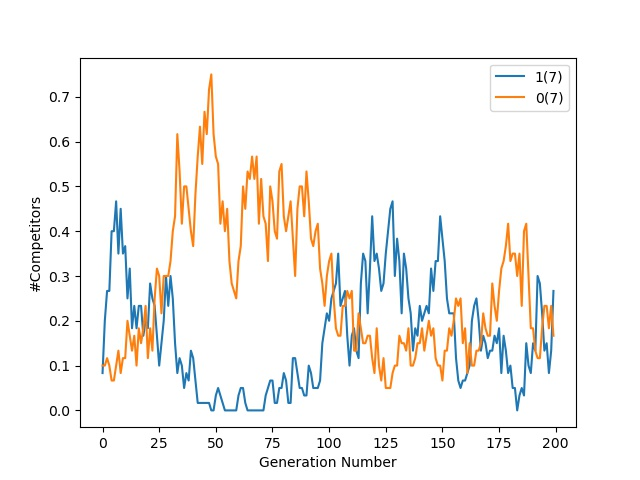
\includegraphics{Codes/Problem_2 Construction_1/Comp_7.jpg} & 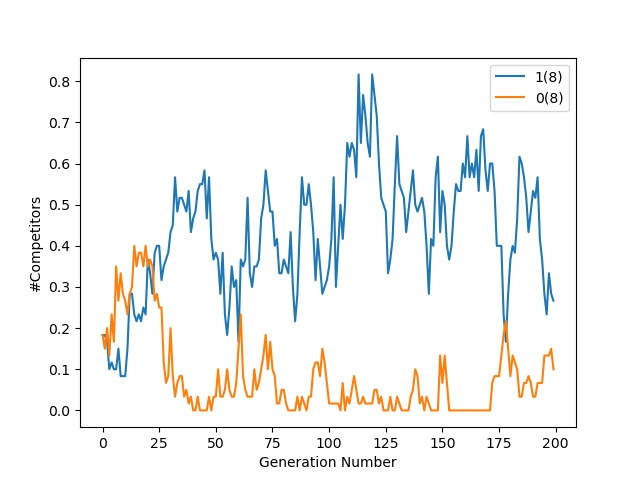
\includegraphics{Codes/Problem_2 Construction_1/Comp_8.jpg} \\
			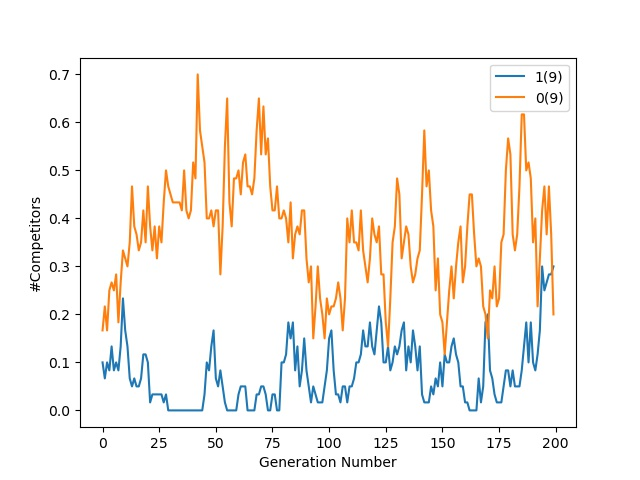
\includegraphics{Codes/Problem_2 Construction_1/Comp_9.jpg}&
			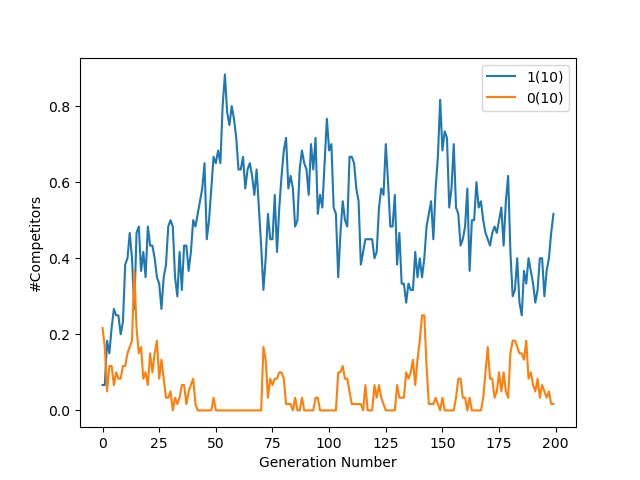
\includegraphics{Codes/Problem_2 Construction_1/Comp_10.jpg}\\
		\end{tabular}
	\end{adjustbox}
	\caption{Plot of fraction of competiting schemas across the generations of the median run. In the legend, 1(x) and 0(x) mean\ all 1s and all 0s for subproblem x respectively.}
	\label{Prob_2_Const_1_Comp_Plot}
\end{figure}

\subsubsection{Construction-2}

Similar to construction 1 of for problem 2, contruction 2 also shows the same trend in terms of objective values and schemas. The objetive scores across the generations are plotted in  \autoref{Prob_2_Const_2_Plot} and the competitor schemas are shown in \autoref{Prob_2_Const_2_Comp_Plot}. 

\begin{figure}[H]
	\centering
	\includegraphics[scale=0.8]{Problem_2 Construction_2/Plot.jpg}
	\caption{The best and average objective scores for the generations of the median run of BGA}
	\label{Prob_2_Const_2_Plot}
\end{figure}    

Here also the algorithm got really confused between selecting 1s and 0s for different subproblems.
	
\begin{figure}[H]
	\centering
	\begin{adjustbox}{width=0.6\paperwidth}
		\begin{tabular}{c c}
			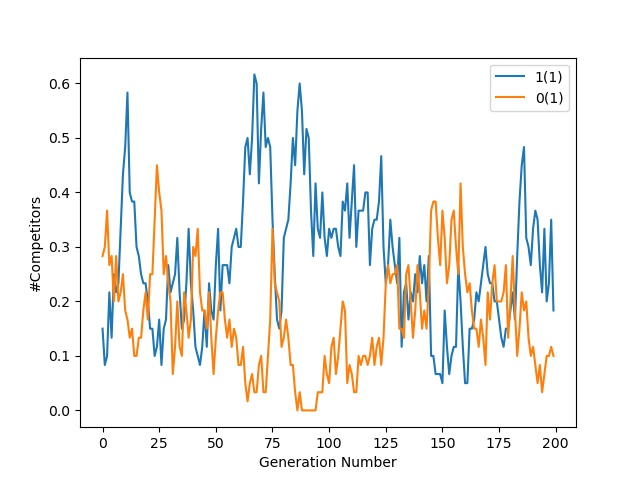
\includegraphics{Codes/Problem_2 Construction_2/Comp_1.jpg} & 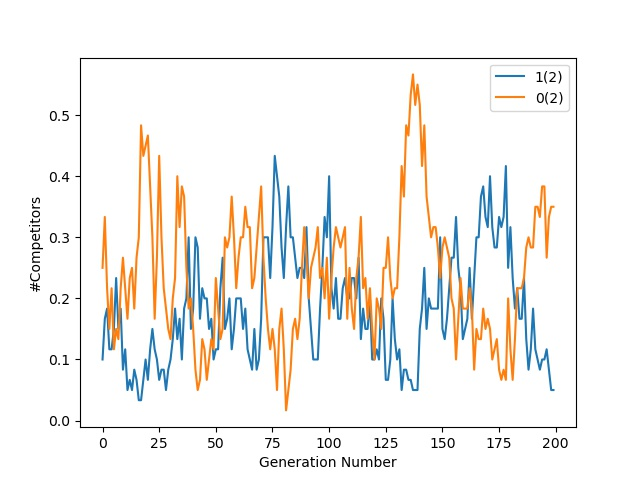
\includegraphics{Codes/Problem_2 Construction_2/Comp_2.jpg} \\
			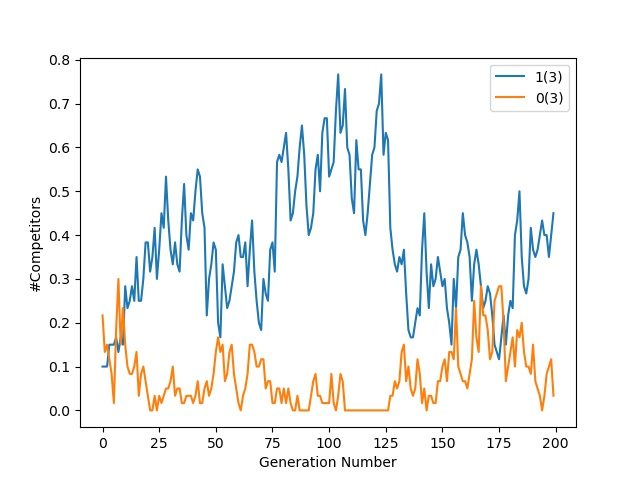
\includegraphics{Codes/Problem_2 Construction_2/Comp_3.jpg}&
			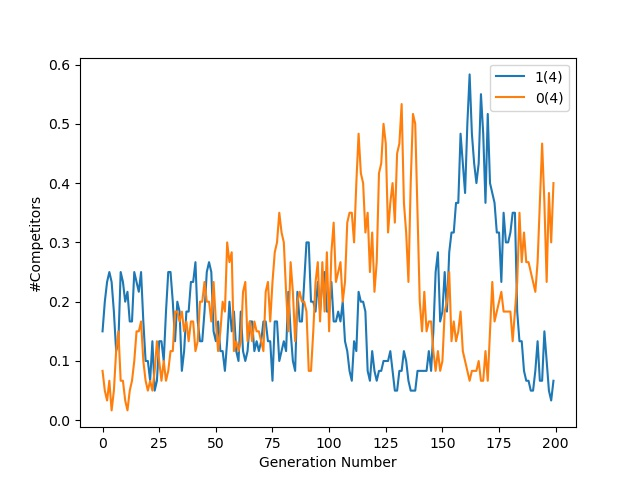
\includegraphics{Codes/Problem_2 Construction_2/Comp_4.jpg} \\ 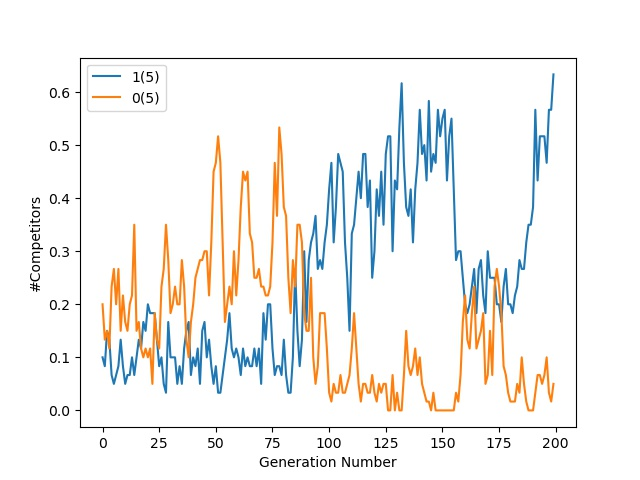
\includegraphics{Codes/Problem_2 Construction_2/Comp_5.jpg} &
			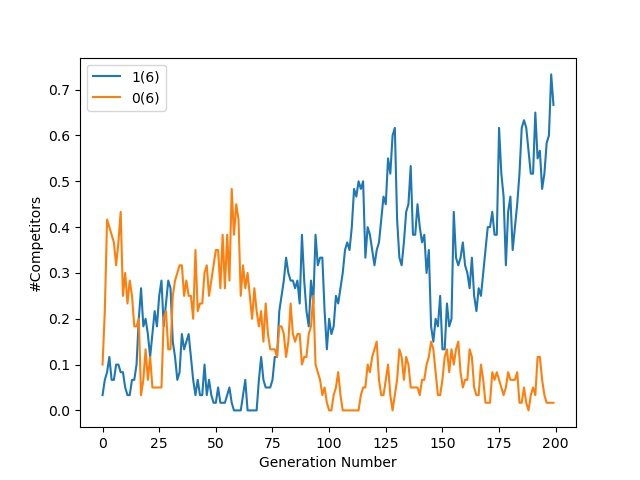
\includegraphics{Codes/Problem_2 Construction_2/Comp_6.jpg}\\
			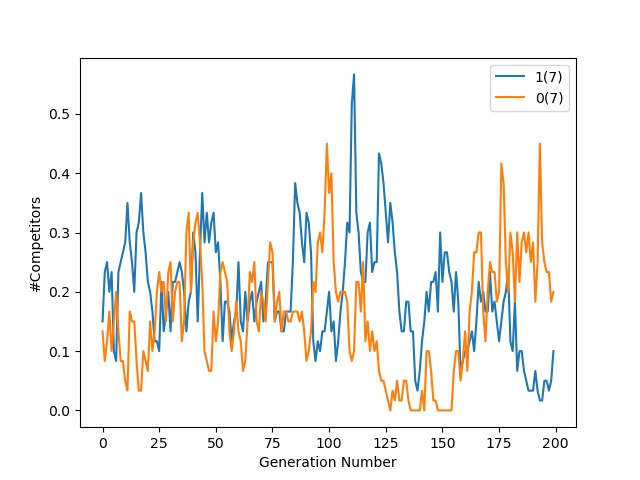
\includegraphics{Codes/Problem_2 Construction_2/Comp_7.jpg} & 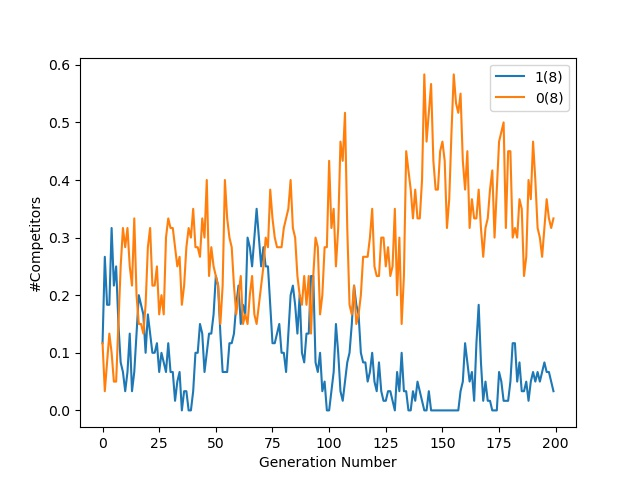
\includegraphics{Codes/Problem_2 Construction_2/Comp_8.jpg} \\
			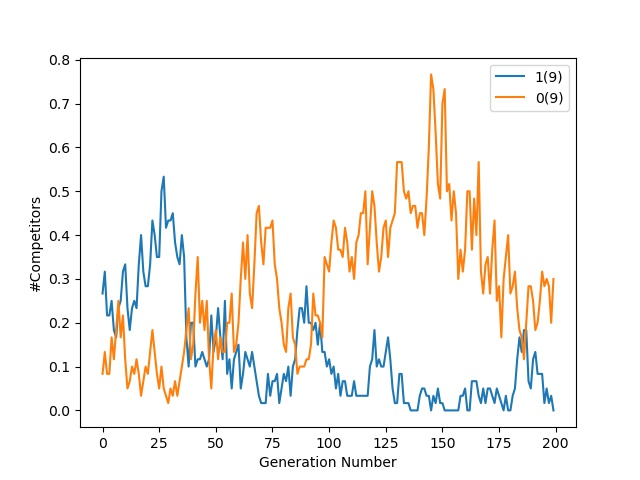
\includegraphics{Codes/Problem_2 Construction_2/Comp_9.jpg}&
			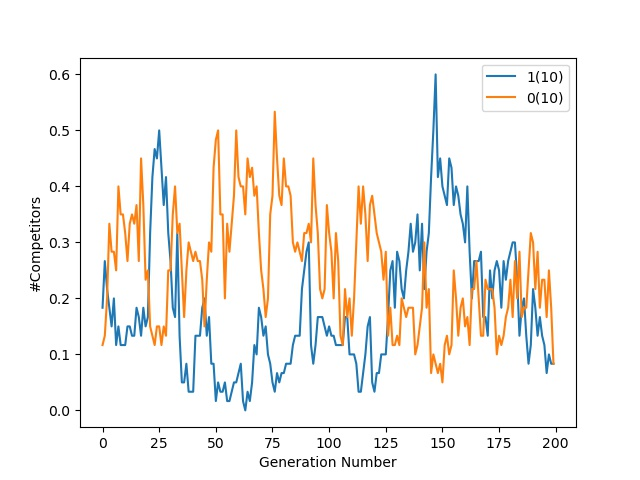
\includegraphics{Codes/Problem_2 Construction_2/Comp_10.jpg}\\
		\end{tabular}
	\end{adjustbox}
	\caption{Plot of fraction of competiting schemas across the generations of the median run. In the legend, 1(x) and 0(x) mean\ all 1s and all 0s for subproblem x respectively.}
	\label{Prob_2_Const_2_Comp_Plot}
\end{figure}

\subsection{Conclusion}
In conclusion, I can say that the BGA implementation is able to find the global maximum solution for problem 1 easily but it is unable to find the same for problem 2. The exploration-exploitation trade-off of BGA can be checked using these 2 problems as problem 1 focuses mostly on exploitation, but problem 2 tests the explorational abilities of the algorithm too. The large crossover rate tries to enhance exploration, but still it was not able to find the global maximum.\\


According to my interpretation, the reason why the BGA could not reach the global maximum solution for problem 2 is because the global maximum solution is not in a stable equilibrium position. So, if even one bit for the global optimum solution gets changed, it deviates a lot in terms of the objective score. Also, one major point in terms of the algorithm is that it does not use elitist preservation. So, even if the global optimum was reached in the mid of the generations, it might get changed easily by the algorithm and would not be preserved due to the absence of the elitist preservation strategy.\\

The competitive schema preservation plots show how the algorithm got confused for problem 2. It is really interesting how the growth in schema can be changed in such a way just for different formulations of the objective function. The solution to this problem is to use separate schemes for the two problems. I think introducing operators like elitist preservations and parent-child comparison can help to solve problem 2.\\ 
\end{document}

